% --------------------------------------------------------------
% This is all preamble stuff that you don't have to worry about.
% Head down to where it says "Start here"
% --------------------------------------------------------------

\documentclass[10pt]{beamer}

% \usepackage[margin=1in]{geometry}
\usepackage{amsmath,amsthm,amssymb,mathrsfs}
\usepackage{tikz}
\usepackage{wrapfig}
\usepackage{cjhebrew}
% \usepackage[shortlabels]{itemize}

\usepackage[utf8]{inputenc}
\usepackage[english]{babel}

\usetikzlibrary{calc}
\usetikzlibrary{arrows.meta}
\usetikzlibrary{arrows}

\title{Optimal Lipschitz Extension Problem}
\author{Aidan Backus}

\newcommand{\NN}{\mathbb{N}}
\newcommand{\ZZ}{\mathbb{Z}}
\newcommand{\QQ}{\mathbb{Q}}
\newcommand{\RR}{\mathbb{R}}
\newcommand{\CC}{\mathbb{C}}


\newcommand*\dif{\mathop{}\!\mathrm{d}}
\DeclareMathOperator*{\argmin}{argmin}
\DeclareMathOperator{\dist}{dist}
\DeclareMathOperator{\Lip}{Lip}
\DeclareMathOperator{\hull}{hull}
\DeclareMathOperator{\Stretch}{stretch}
\DeclareMathOperator{\supp}{supp}
\DeclareMathOperator{\Var}{Var}
\DeclareMathOperator{\Exc}{Exc}
\DeclareMathOperator*{\Expect}{\mathbf E}
\newcommand{\normal}{\vec n}
\newcommand{\id}{\mathrm{id}}
\newcommand{\norm}[1]{\left\lVert#1\right\rVert}

\newcommand{\Spec}{\operatorname{Spec}}

\renewcommand{\Re}{\operatorname{Re}}
\renewcommand{\Im}{\operatorname{Im}}

\newtheorem{theoremconjecture}{Theorem-Conjecture}
\newtheorem{conjecture}{Conjecture}
\newtheorem{proposition}{Proposition}
\newtheorem{question}{Question}

\usepackage[backend=bibtex,style=alphabetic,maxcitenames=50,maxnames=50]{biblatex}
\addbibresource{ultrapowerful.bib}
\renewbibmacro{in:}{}
\DeclareFieldFormat{pages}{#1}

\usetheme{AnnArbor}
\usecolortheme{dove}

% \setbeamertemplate{itemize item}{\usebeamerfont*{itemize item}\raise1.25pt\hbox{\donotcoloroutermaths$\bullet$}}
% \setbeamertemplate{itemize subitem}[triangle]
% \setbeamertemplate{itemize subsubitem}[square]

\begin{document}
% --------------------------------------------------------------
%                         Start here
% --------------------------------------------------------------
\frame{\titlepage}

\begin{frame}{Lipschitz maps}
\begin{definition}
Let $f: X \to Y$ be a mapping between metric spaces and $A \subseteq X$ a set.
The \emph{Lipschitz constant} of $f$ on $A$ is
$$\Lip(f, A) := \sup_{x, y \in A} \frac{\dist_Y(f(x), f(y))}{\dist_X(x, y)}.$$
\end{definition}
 
\begin{problem}
Given a set of Lipschitz mappings $\mathscr F$, find one which is ``optimal''.
\end{problem}
\end{frame}

\begin{frame}{Motivation from Teichm\"uller theory}
\begin{itemize}
\item Let $S$ be a closed surface of Euler characteristic $\chi \leq -2$. 
\begin{itemize}
\item By the Gauss-Bonnet theorem, any Riemannian metric $g$ on $S$ with curvature $K_g$ satisfies 
$$\int_S K_g ~\dif A_g = 2\pi \chi \leq -4\pi,$$
so it is natural to look for $g$ with $K_g = -1$ -- in other words $g$ is \emph{hyperbolic}.
\item There are too many hyperbolic metrics, so we search for a way to understand them en masse. 
\end{itemize}
\item If $g, h$ are hyperbolic metrics, their \emph{Thurston distance} is
$$\dist(g, h) = \inf_{f \sim \id_S} \log \Lip_{(S, g) \to (S, h)}(f, S).$$
\begin{itemize}
\item This metric encodes how geodesics on $(S, g)$ deform when $g$ is deformed (Thurston '86, Papadopoulos '15, Gu\'eritaud and Kassel '17, Daskalopoulos and Uhlenbeck '24...) 
\end{itemize}
\end{itemize}
\end{frame}

\begin{frame}{The Kirszbraun-Valentine theorem}
\begin{itemize}
\item We're going to focus on euclidean space in these lectures.
\begin{itemize}
\item Many of these results extend to Riemannian manifolds, and in particular have applications to understanding deformations of hyperbolic surfaces. 
\end{itemize}
\item First attempt: Find a Lipschitz mapping which minimizes its Lipschitz constant. 
\end{itemize}
'
\begin{theorem}[Kirszbraun-Valentine theorem]
Let $K$ be a compact subset of $\RR^d$ and $f: K \to \RR^D$ a Lipschitz mapping.
Then there exists $u: \RR^d \to \RR^D$ such that: 
\begin{itemize}
\item $u|_K = f$, 
\item and $\Lip(u, \RR^d) = \Lip(f, K)$.
\end{itemize}
\end{theorem}
\end{frame}

\begin{frame}{Proving the Kirszbraun-Valentine theorem}
\begin{lemma}[Gu\'erituad and Kassel '17]
Let $K$ be a compact subset of $\RR^d$, $f: K \to \RR^D$ a Lipschitz mapping, and $x \notin K$.
For each $\xi \in \RR^D$, let 
$$\varphi(\xi) := \max_{y \in K} \frac{|\xi - f(y)|}{|x - y|}.$$
Then: 
\begin{itemize}
\item There exists a minimum $\xi^*$ of $\varphi$. 
\item Let $K'$ be the set of all $y \in K$ such that $|\xi - f(y)| = \varphi(\xi^*) |x - y|$. Then: 
\begin{itemize}
\item $\xi^* \in \hull(f(K'))$. 
\item There exist $y_1, y_2 \in K'$ such that 
$$\angle(y_1, x, y_2) \leq \angle(f(y_1), \xi^*, f(y_2)),$$
and the latter angle is not zero.
\end{itemize}
\end{itemize}
\end{lemma}
\end{frame}

\begin{frame}{Proving the Kirszbraun-Valentine theorem}
\begin{lemma}
Let $K$ be a compact subset of $\RR^d$, $f: K \to \RR^D$ a Lipschitz mapping, and $x \notin K$.
Then
$$\min_{\xi \in \RR^d} \max_{y \in K} \frac{|\xi - f(y)|}{|x - y|} \leq \Lip(f, K).$$
\end{lemma} 

\begin{itemize}
\item We prove the Kirszbraun-Valentine theorem by iterating this lemma. 
\item Since the only property of euclidean geometry that we used is triangle comparison, this can be made to work in more general metric spaces with bounds on their Alexandrov curvature.
\end{itemize}
\end{frame}

\begin{frame}{A failure of uniqueness}
    \centering 
    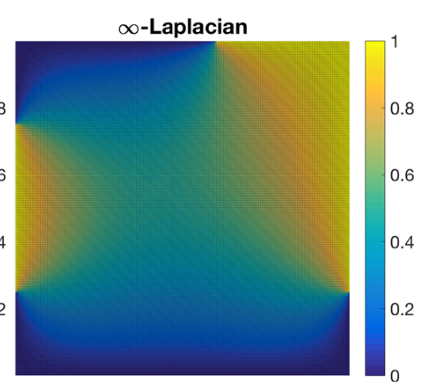
\includegraphics[width=6cm]{KirszbraunValentine.png}
    
\begin{itemize}
\item Adapted from Loisel '20: A minimizing Lipschitz function.  
\item Since the function is nearly constant near the upper-left corner, we can add artificial oscillations there to break uniqueness.
\end{itemize}
\end{frame}

\begin{frame}{Absolutely minimizing Lipschitz mappings}
\begin{itemize}
\item The problem is that variational problems defined by integrals already locally minimize, but not $L^\infty$ variational problems. 
\item Second attempt: Try a more localized version of the Lipschitz minimization property. 
\end{itemize}

\begin{definition}
Let $U \subseteq \RR^d$ be an open set.
A mapping $u: U \to \RR^D$ is \emph{absolutely minimizing Lipschitz} (\emph{AML}) if 
\begin{itemize}
\item for every open set $V \subseteq \RR^d$ of sufficiently small diameter, 
\item and every $v: V \to \RR^D$ with $\Lip(v, \partial V) = \Lip(u, \partial V)$, 
\end{itemize}
one has
$$\Lip(u, V) \leq \Lip(v, V).$$
\end{definition}
\end{frame}

\begin{frame}{Well-posedness of AML scalar fields}
\begin{itemize}
\item In general, AML mappings are too hard, but AML scalar fields are easier. 
\item Recall the $p$-Laplacian 
$$\Delta_p u := \nabla \cdot (|\nabla u|^{p - 2} \nabla u) = 0$$
whose solutions minimize $\|\nabla u\|_{L^p}$. 
\item Aronsson '67: Since $\|\nabla u\|_{L^p} \to \Lip(u, U)$ as $p \to \infty$, study $p$-harmonic functions as $p \to \infty$. 
\end{itemize}

\begin{theorem}[Jensen '93]
Let $U \subseteq \RR^d$ be an open set with Lipschitz boundary, and $f: \partial U \to \RR$ a Lipschitz function. Then: 
\begin{itemize}
\item There is a unique AML function $u: U \to \RR$ such that $u|_{\partial U} = f$. 
\item Let $u_p$ be the unique $p$-harmonic extension of $f$.
Then $u_p \to u$ in $C^0$ as $p \to \infty$.
\end{itemize}
\end{theorem}
\end{frame}

\begin{frame}{The $\infty$-Laplacian}
\begin{itemize}
\item The $p$-Laplacian is quasilinear and its solutions are only $C^{1 + \alpha}$.
\begin{itemize}
\item In Aronsson's time, the $p$-Laplacian could only be understood in divergence form: for every $\varphi \in C^\infty_c(U)$,
$$\int_U \langle \nabla \varphi, |\nabla u|^{p - 2} \nabla u\rangle \dif V = 0.$$
\end{itemize}
\item Pretend for a moment that we could legally write the $p$-Laplacian in nondivergence form 
$$(p - 2) |\nabla u|^{p - 4} \langle \nabla^2 u, \nabla u \otimes \nabla u\rangle + |\nabla u|^{p - 2} \Delta u = 0.$$
Renormalize and take $p \to \infty$ to find the limiting PDE: 
\end{itemize} 

\begin{definition}
The \emph{$\infty$-Laplacian} is the PDE 
$$\Delta_\infty u := \langle \nabla^2 u, \nabla u \otimes \nabla u\rangle = 0.$$
\end{definition}
\end{frame}

\begin{frame}{Classical solutions of the $\infty$-Laplacian}
\begin{itemize}
\item Affine functions.
\item $|x|$, on the punctured space.
\item $x_1^{4/3} - x_2^{4/3}$, on Quadrant I.
\item $\arctan(x_2/x_1)$, on the Riemann surface of $\log$.
\item Classical solutions of the eikonal equation $|\nabla u| = \lambda$.
\end{itemize}
\end{frame}

\begin{frame}{The $\infty$-Laplacian is a horrible PDE}
\begin{itemize}
\item $\Delta_\infty$ is totally nonlinear, and only elliptic in the $\nabla u$ direction.  
\begin{itemize}
\item So $u$ should not have much more regularity than Lipschitz. 
\item $x^{4/3} - y^{4/3}$ is AML, but is only $C^{1 + 1/3}$. 
\item According to Evans and Smart '11, in $d = 2$ you should think of $\Delta_\infty$ as a totally nonlinear parabolic PDE where the time vector field is $\nabla^2 u \cdot \nabla u$ and the space vector field is $\nabla u$. 
\end{itemize}
\item We cannot define solutions using integration by parts. 
\begin{itemize}
\item $\Delta_\infty$ cannot be written in divergence form. 
\item So Aronsson got stuck here.
\end{itemize}
\end{itemize}
\end{frame}

\begin{frame}{The miracle on the viscosity-ula}
\begin{itemize}
\item The correct solution concept was introduced by Crandall, Evans, and Lions '84 in their work on Hamilton-Jacobi equations. 
\item Too hard to motivate for the $\infty$-Laplacian a priori, so let's do it for inviscid Burgers' equation first:
$$\partial_t u + u \partial_x u = 0.$$
This has way too many solutions!  
\item The physically correct solutions are $C^0$ limits of the viscous problem 
$$\partial_t u + u \partial_x u = \varepsilon \partial_x^2 u.$$
This is a semilinear parabolic PDE, so it satisfies the maximum principle: 
\begin{itemize}
\item If $v \in C^2$ and $u - v$ has a local maximum at $(x_*, t_*)$, then
$$\partial_t v(x_*, t_*) + v(x_*, t_*) \partial_x v(x_*, t_*) \leq \varepsilon \partial_x^2 v(x_*, t_*).$$
\end{itemize}
\end{itemize}
\end{frame}

\begin{frame}{Viscosity solutions of inviscid Burgers}
\begin{itemize}
\item The maximum principle is a result about pointwise comparison, so it's preserved by $C^0$ limits. 
\item So, if $u$ is a solution of inviscid Burgers which is physically meaningful, it is a viscosity solution: 
\end{itemize}

\begin{definition}
Let $u \in C^0((-T, T) \times \RR)$. We say that $u$ is a \emph{viscosity solution of inviscid Burgers' equation} if, for every $v \in C^1((-T, T) \times \RR)$:  
\begin{itemize}
\item If $u - v$ has a local maximum at $(x_*, t_*)$, then
$$\partial_t v(x_*, t_*) + v(x_*, t_*) \partial_x v(x_*, t_*) \leq 0.$$
\item If $u - v$ has a local minimum at $(x_*, t_*)$, then 
$$\partial_t v(x_*, t_*) + v(x_*, t_*) \partial_x v(x_*, t_*) \geq 0.$$
\end{itemize}
\end{definition}
\end{frame}

\begin{frame}{Viscosity solutions of the $\infty$-Laplacian}
\begin{lemma}[maximum principle for the $p$-Laplacian]
Suppose that $U$ is an open set with Lipschitz boundary, $\Delta_p u \geq 0$, and $\Delta_p v \leq 0$, and $u \leq v$ on $\partial U$.
Then $u \leq v$ on $U$.
\end{lemma}   
 
\begin{definition}
Let $u \in C^0(U)$. Then:
\begin{itemize}
\item $u$ is \emph{$\infty$-subharmonic} at $x_* \in U$ (or that $\Delta_\infty u \geq 0$ \emph{in the sense of vanishing viscosity}), if, for every $v \in C^2(U)$ such that $u - v$ has a local maximum at $x_*$,
$$\Delta_\infty v(x_*) \geq 0.$$
\item $u$ is \emph{$\infty$-superharmonic} if $-u$ is $\infty$-subharmonic.
\item $u$ is \emph{$\infty$-harmonic} if $u$ is $\infty$-subharmonic and $\infty$-superharmonic.
\end{itemize}
\end{definition}
\end{frame}

\begin{frame}{Existence}
\begin{lemma}
Let $U \subset \RR^d$ have a Lipschitz boundary, and let $f$ be a Lipschitz function on $\partial U$.
Let $1 < p, r < \infty$, and let $u_p$ be the $p$-harmonic extension of $f$. Then
$$\|\nabla u_p\|_{L^r} \leq \operatorname{vol}(U)^{1/r} \Lip(f, \partial U) .$$
\end{lemma}
 
\begin{proposition}
Let $U \subset \RR^d$ have a Lipschitz boundary and finite volume, and let $f$ be a Lipschitz function on $\partial U$.
Then there is an $\infty$-harmonic extension $u$ of $f$. Moreover,
$$\Lip(u, U) = \Lip(f, \partial U).$$
\end{proposition}
\end{frame}

\begin{frame}{Uniqueness}
\begin{theorem}[Jensen's maximum principle]
Suppose that $u$ is $\infty$-subharmonic and $v$ is $\infty$-superharmonic on $U$.
If $u \leq v$ on $\partial U$, then $u \leq v$.
\end{theorem}

\begin{lemma}
Suppose that $u$ is $\infty$-subharmonic on $U$, and $\varepsilon > 0$.
Then there is an $\infty$-subharmonic function $u_\varepsilon$, such that: 
\begin{itemize}
\item $u_\varepsilon = u$ on $\{|\nabla u| \geq \varepsilon\} \cup \partial U$, but  
\item on $\{|\nabla u| < \varepsilon\}$, $u_\varepsilon$ is a viscosity solution of the eikonal equation $|\nabla u_\varepsilon| = \varepsilon$.
\end{itemize}
\end{lemma}
\end{frame}

\begin{frame}{Regularity}
\begin{theorem}
Let $u$ be $\infty$-harmonic. Then: 
\begin{itemize}
\item (Evans and Savin '08) If $d = 2$, then for some $\alpha > 0$, $u \in C^{1 + \alpha}$. 
\item (Evans and Smart '11) $u$ is differentiable. 
\end{itemize}
\end{theorem}

\begin{itemize}
    \item Idea behind Evans and Savin: Do a highly anisotropic blowup, since $\Delta_\infty$ only looks elliptic in the $\nabla u$ direction.
\end{itemize}

\begin{problem}
    What is the sharp regularity of $\infty$-harmonic functions?
\end{problem}

\begin{problem}
    Let $u$ be a $C^2$ $\infty$-harmonic function on a domain in $\RR^2$, such that $|\nabla^2 u \nabla u| \geq \varepsilon$.
    If $v$ is an $\infty$-harmonic function and a small perturbation of $u$, can we get higher regularity for $v$?
\end{problem}
\end{frame}

\begin{frame}{Comparison with cones}

\begin{itemize}
\item By Jensen's maximum principle applied to the punctured ball, if $u$ is $\infty$-subharmonic, $u(0) = 0$, and $|x| = r$ implies $u(x) \leq |x|$, then $|x| \leq r$ implies $u(x) \leq |x|$. 
\end{itemize}

\begin{definition}
A function $u \in C^0(U)$ satisfies: 
\begin{itemize}
\item \emph{comparison with cones from above}, if for every $B(x_*, r) \Subset U$, if $u(x) \leq u(x_*) + B|x - x_*|$ for $x \in \partial B(x_*, r)$, then the same inequality holds for $x \in B(x_*, r)$.
\item \emph{comparison with cones}, if $u$ and $-u$ both satisfy comparison with cones from above. 
\end{itemize}
\end{definition}

\begin{proposition}
A function $u \in C^0(U)$ is $\infty$-subharmonic iff $u$ satisfies comparison with cones from above.
\end{proposition}
\end{frame}

\begin{frame}{Characterization of $\infty$-harmonic functions}
\begin{theorem}
Let $U \subseteq \RR^d$ be a bounded Lipschitz domain.
The following are equivalent for $u \in C^0(U)$: 
\begin{enumerate}
\item $u$ is $\infty$-harmonic. 
\item $u$ satisfies comparison with cones. 
\item $u$ is absolutely minimizing Lipschitz. 
\item $u$ is the limit in $C^0$ of $p$-harmonic functions as $p \to \infty$. 
\item $u$ is the limit in $C^0$ of values of tug-of-war games at scale $\varepsilon$, as $\varepsilon \to 0$. 
\end{enumerate}
\end{theorem}
    
\begin{itemize}
    \item We showed that 1, 2, and 4 are equivalent. 
    \item Let us show that 2 is equivalent to 3. 
    \item If we have time we will define 5 and sketch the proof that 3 is equivalent to 5.
\end{itemize}
\end{frame}

\begin{frame}{Tug of war}
\begin{itemize}
\item Let $(X, E)$ be an (undirected, unweighted, possibly infinite) graph and $Y \subset X$. 
\item Introduce \emph{Alice's payoff for tug-of-war} $f: Y \to \RR$.  
\begin{itemize}
\item Alice and Bob are going to play a game where the set of game states is $X$, and the set of terminal game states is $Y$.
\item If the final game state is $y \in Y$, Bob will pay Alice $f(y)$.  
\end{itemize}
\item Suppose that the game is in state $x \in X$.  
\begin{itemize}
\item Alice flips a coin.
\item If it's heads, it's Alice's turn. Otherwise it's Bob's turn.
\item The player whose turn it is moves the game to a state $x'$ adjacent to $x$.
\item If $x' \in Y$, the game ends.
\end{itemize}
\end{itemize}
\end{frame}

\begin{frame}{Strategies}
\begin{itemize}
\item A \emph{strategy for tug-of-war} is a mapping which sends $x \in X$ to a probability distribution on the set of vertices adjacent to $x$. 
\begin{itemize} 
\item Suppose that Alice's strategy is $S$, the game is in state $x$, and Alice won the coin toss. 
\item Then Alice uses the probability distribution $S(x)$ to draw a vertex $x'$ adjacent to $x$ at random.
\item Alice then moves the game state to $x'$. 
\end{itemize}
\item \emph{Alice's value function for tug-of-war} $u(x)$ at $x \in X$ is
\begin{itemize}
\item the supremum over all strategies $S_{\rm Alice}$
\item of the infimum over all strategies $S_{\rm Bob}$
\item of the expected value of Alice's payoff $f(y)$, where $y$ is the end state of the game such that:
\begin{itemize}
\item the initial state of the game was $x$, and
\item Alice and Bob played the strategies $S_{\rm Alice}$ and $S_{\rm Bob}$.
\end{itemize}
\end{itemize}
\end{itemize}
\end{frame}

\begin{frame}{Dynamic programming}
\begin{itemize}
\item Alice's optimal strategy is to always move in a direction which increases her value function as much as possible. 
\item However, she only has a half-chance to move, and otherwise (if he is playing optimally) Bob will decrease Alice's value function as much as possible.  
\end{itemize}

\begin{proposition}
Let $u$ be Alice's value function for tug-of-war. Then 
$$u(x) = \frac{1}{2} \left[\sup_{x_{\rm Alice} \sim x} u(x_{\rm Alice}) + \inf_{x_{\rm Bob} \sim x} u(x_{\rm Bob})\right].$$
\end{proposition}  

\begin{itemize}
\item The finite difference equation for $u$ looks suspiciously like the $\infty$-Laplacian... 
\end{itemize}
\end{frame}

\begin{frame}{Tug-of-war at scale $\varepsilon$}
\begin{definition}
Let $X$ be a metric space, $Y \subset X$, $\varepsilon > 0$, and $\{x, x'\} \in E$ iff $\dist(x, x') < \varepsilon$.
Then \emph{tug-of-war at scale $\varepsilon$} on $X$ is the game just described with the graph $(X, E)$ and set of final states $Y$.
\end{definition} 

\begin{theorem}[Peres, Schramm, Sheffield, and Wilson '08]
Suppose that $X$ is a length space and $Y \subset X$ is nonempty.
Let $f: Y \to \RR$ be bounded Lipschitz function with a uniformly continuous extension to $X$.
Then: 
\begin{itemize}
\item Let $f$ be Alice's payoff for a game of tug-of-war at scale $\varepsilon$.
Then Alice's value function $u_\varepsilon$ is well-defined and uniformly continuous on $X$.  
\item There exists an AML function $u$ such that $\|u - u_\varepsilon\|_{C^0} \lesssim \varepsilon$. 
\end{itemize}
\end{theorem}
\end{frame}

\begin{frame}{Geodesic laminations}
\begin{definition}
A \emph{geodesic lamination} is a closed set $\lambda \subseteq U$ equipped with a partition of $\lambda$ into line segments $\gamma$, called \emph{leaves}, such that $\partial \gamma \subseteq \partial U$. 
\end{definition}

\begin{itemize}
\item Mainly studied in hyperbolic surfaces. A picture from Thurston '97 in that case:
\end{itemize}

\centering 
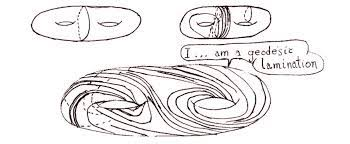
\includegraphics[width=7cm]{GeodesicLamination.jpg}
    
\end{frame}

\begin{frame}{The geodesic lamination in the stretch set}
\begin{theorem}[Daskalopoulos and Uhlenbeck '20]
Let $u$ be an $\infty$-harmonic function on $U$ such that $\Stretch(u, U)$ is nonempty.
Then $\Stretch(u, U)$ is a geodesic lamination, and for any leaf $\gamma \subseteq \Stretch(u, U)$,
$$\frac{\dif}{\dif t} u(\gamma(t)) = \Lip(u, U).$$
\end{theorem}
\end{frame}

\begin{frame}{The dual problem}
\begin{theorem}[Daskalopoulos and Uhlenbeck '20]
Suppose that $d = 2$, and $u_p$ are $p$-harmonic functions on $U$ converging to an $\infty$-harmonic function $u$.
Let $v_q$ be the dual $q$-harmonic harmonic to $u_p$.
Then:
\begin{itemize}
\item $v_q$ converges in the weakstar topology of $BV$ to a function $v$ of least gradient.
\item If $v$ is not constant, then $\dif v$ is a transverse measure to $\Stretch(u, U)$.
\end{itemize}
\end{theorem}
\end{frame}

\begin{frame}{Some problems in Daskalopoulos and Uhlenbeck '20}
\begin{problem}
Verify that the theory of $\infty$-harmonic functions goes through unchanged on a (simply connected) Riemannian manifold.
(More generally, is there a class of ``$\infty$-elliptic'' PDE which satisfy, for example, the Evans--Savin theorem?)
\end{problem}

\begin{problem}
Let $M$ be a closed oriented Riemannian manifold, and let $\rho$ be a homotopy class of maps from $M$ to the circle.
Show that there is a unique $\infty$-harmonic map representing $\rho$.
\end{problem}
\end{frame}

\begin{frame}{Nonuniqueness of AML mappings}
    Too many holomorphic functions...
\end{frame}

\begin{frame}{A toy problem on graphs}
    Lexicographic minimizers
\end{frame}

\begin{frame}{Sheffield and Smart's formulation}
\begin{theorem}[Sheffield and Smart '10]
Let $u: U \to \RR^D$ be a smooth mapping such that $\xi$ is the unique principal singular vector of $\nabla u$.
Then $u$ is tight iff 
$$\langle \nabla \langle \nabla u, \xi\rangle, \xi\rangle = 0.$$
\end{theorem}

\begin{theorem}[Sheffield and Smart '10]
Suppose that $U \subseteq \CC$, and let $u: U \to \CC$ be an injective holomorphic function.
Then $u$ is tight iff the mean curvature of every level set of $\log(Lu^{-1})$ is nonnegative.
\end{theorem}
    
\end{frame}

\begin{frame}{Daskalopoulos and Uhlenbeck's formulation}
    
\end{frame}

\begin{frame}{$W^{2, 2}$ estimates break our hearts}
\begin{theorem}[Daskalopoulos and Uhlenbeck '22] 
Suppose that $d = 2$, $4 \leq p < \infty$ and $u_p: U \to \RR^2$ is the $p$-harmonic extension of a Lipschitz map $f$.
Then $\|\nabla^2 u_p\|_{L^2} \lesssim_f 1$.
\end{theorem}
 
\begin{itemize}
\item So $\nabla u_p$ converges to the $\infty$-harmonic map $u$ in the weakstar topology of $BMO$ and the strong topology of $L^r$, $1 < r < \infty$.  
\item If we knew that $\|\nabla u_p - \nabla u\|_{L^r} \ll 1$ independently of $r$, then we could conclude that $u$ is AML, but this estimate appears to be sharp, and is just short of what we need.
\end{itemize}

\end{frame}

\begin{frame}{Comparing the two approaches}
    
\end{frame}

\begin{frame}{The toy model}

\end{frame}

\begin{frame}{A counterexample from contact geometry}
    \begin{itemize}
        \item There is a natural map of spheres $\mathbb S^3 \to \mathbb S^2$, called the \emph{Hopf fibration}, such that the preimage of any point in $\mathbb S^2$ is a great circle. 
    \end{itemize}

    \begin{example}[B '24]
    Let $F$ be the unit $2$-form on $\mathbb S^3$ such that $F(x)$ is conormal to the great circle through $x$ arising from the Hopf fibration.
    Then: 
\begin{itemize}
    \item $F$ solves the tight PDE.  
    \item $F$ does not minimize its $L^\infty$ norm even globally.
\end{itemize}
\end{example}

\begin{itemize}
\item Key point: $F$ is not the area form of any surface.  
\item Thinking of Jensen's maximum principle purely as a uniqueness theorem (rather than a comparison theorem):  
\begin{itemize}
\item There can be no generalization of Jensen's maximum principle to $L^\infty$ variational systems.
\end{itemize}
\end{itemize}
\end{frame}

\begin{frame}{The divide-and-conquer scheme}
    
\end{frame}

\end{document}
